% !TeX program = xelatex
% !TeX encoding = utf8
\documentclass[xetex, onlymath, handout]{beamer}
\usefonttheme{serif}
\usetheme{hsr}

% use lmodern for math
\usepackage{lmodern}

%% Pretty figures
\usepackage{circuitikz}  % Electric diagrams
\usepackage{pgfplots}    % Pretty plots
\usepackage{tikz}        % Pretty drawings
\usepackage{tikz-3dplot} % More dimensions!

\usetikzlibrary{
	external,
	calc,
	positioning,
	backgrounds,
	decorations.pathreplacing,
	calligraphy,
	decorations.markings,
	matrix,
	arrows,
	patterns,
}
\pgfplotsset{compat=newest}

% math packages
\usepackage{amsmath}
\usepackage{amssymb}

\usepackage[T1]{fontenc}
\usepackage{beramono} % monospaced
\usepackage{roboto} % other
\renewcommand*\familydefault{\sfdefault}

% metadata
\title{Multipath Fading Demonstration Platform using Software Defined Radio}
\author{Naoki Sean Pross \and Sara Cinzia Halter}
\date{23. December 2021}

\institute[OST]{OST FHO Campus Rapperswil}

\AtBeginSection[]
{
  \begin{frame}{Table of Contents}
    \tableofcontents[currentsection]
  \end{frame}
}


\begin{document}

\frame{
  \maketitle
}

\section{Multipath Fading}

\begin{frame}{Multipath Fading sketch}
	\begin{figure}
		\centering
		% vim: set ts=2 sw=2 noet:
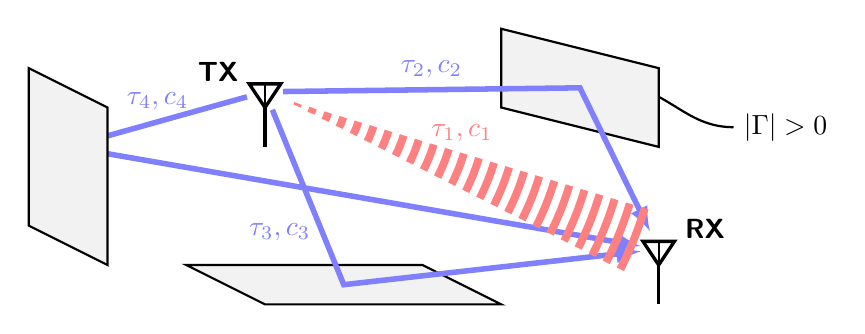
\begin{tikzpicture}[
			antenna/.pic = {
				\draw[very thick] (0,0) -- ++(2mm, 3mm) -- ++(-4mm,0) -- cycle;
				\draw[very thick] (0,0) -- ++(0,-5mm) coordinate (-mast) {};
				\draw[thick] (0,0) -- ++(0,3mm);
				\node[inner sep = 0pt, outer sep = 6pt] (-center) at (0,2mm) {};
			},
	]

	% Antennas
	\draw (0,2) pic (T) {antenna} node[above left = 3mm] {\sffamily\bfseries TX};
	\draw (5,0) pic (R) {antenna} node[above right = 3mm] {\sffamily\bfseries RX};

	% wall coefficients
	\draw[thick] (4.75, 2.25) to[out = -20, in = 180] ++(1.2,-.5) node[right] {\(|\Gamma| > 0\)};

	% walls
	\draw[thick, fill = lightgray!20] (3,2) -- ++(2,-.5) -- ++(0,1) -- ++(-2,.5) -- cycle;
	\draw[thick, fill = lightgray!20] (-1,0) -- ++(3,0) -- ++(1,-.5) -- ++(-3,0) -- cycle;


	% reflected signals
	\draw[line width = 2pt, blue!50!white, -latex] (T-center) -- node[above, pos = .5] {\(\tau_2,c_2\)} (4,2.25) -- (R-center);
	\draw[line width = 2pt, blue!50!white, -latex] (T-center) -- node[left, pos = .7] {\(\tau_3,c_3\)} (1,-.25) -- (R-center);
	\draw[line width = 2pt, blue!50!white, -latex] (T-center) -- node[above, pos = .5] {\(\tau_4,c_4\)} (-2.5,1.5) -- (R-center); 

	% another wall
	\draw[thick, fill = lightgray!20] (-2,0) -- ++(-1,.5) -- ++(0,2) --++(1,-.5) -- cycle;

	% LOS path
	\draw[line width = 1mm, red!50!white,
		decorate, decoration = {
			expanding waves, angle = 5, segment length = 2mm
		}
	] (T-center) -- node[above = 2mm, pos = .5] {\(\tau_1,c_1\)} (R-center);
\end{tikzpicture}

	\end{figure}
	\begin{equation} \label{eqn:multipath-impulse-response}
		h(\tau, t) = \sum_k c_k(t) \delta(\tau - \tau_k(t)),
	\end{equation}
\end{frame}

\begin{frame}{Spectrum of a multipath fading channel}
	\begin{figure}
		\centering
		\resizebox{\linewidth}{!}{
			% vim: set ts=2 sw=2 noet:
\begin{tikzpicture}
	\begin{loglogaxis}[
			width = .6\linewidth, height = 5cm,
			ylabel = {Response \(|H(f, t)|\)},
			xlabel = {Frequency \(f\)/Hz},
			xlabel near ticks,
			ylabel near ticks,
			ytick = \empty,
			smooth,
		]

		\addplot[solid, magenta] table[x index = 0, y index = 2]
			{figures/data/multipath_frequency_response.dat};
		\addlegendentry{Multipath}

		\addplot[dashed, thick, black] table[x index = 0, y index = 1]
			{figures/data/multipath_frequency_response.dat};
		\addlegendentry{Linear}

	\end{loglogaxis}
\end{tikzpicture}
\hskip 5mm
\begin{tikzpicture}[
		decorated/.style = {
			solid, thick,
			postaction={decorate},
			decoration={markings,
				mark=at position 0.35 with {\arrow{stealth}},
				mark=at position 0.65 with {\arrow{stealth}}},
		},
	]
	\begin{axis}[
			width = 5cm, height = 5cm,
			ylabel = {\(\Im{H(f,t)}\)},
			xlabel = {\(\Re{H(f,t)}\)},
			xlabel near ticks,
			ylabel near ticks,
			grid = major,
			xmin = -1.2, xmax = 1.2,
			ymin = -1.2, ymax = 1.2,
		]

		\addplot[decorated, red] table[x index = 3, y index = 4]
			{figures/data/multipath_frequency_response.dat}
			node[pos = 0, circle, fill = white, draw, inner sep = 1pt] {}
			node[pos = .2, outer sep = 1pt, inner sep = 0pt] (A) {}
			node[pos = 1, circle, fill = white, draw, inner sep = 1pt] {};

		\addplot[decorated, blue] table[x index = 5, y index = 6]
			{figures/data/multipath_frequency_response.dat}
			node[pos = 0, circle, fill = white, draw, inner sep = 1pt] {}
			node[pos = .2, outer sep = 1pt, inner sep = 0pt] (B) {}
			node[pos = 1, circle, fill = white, draw, inner sep = 1pt] {};

		\addplot[decorated, magenta] table[x index = 7, y index = 8]
			{figures/data/multipath_frequency_response.dat}
			node[pos = 0, circle, fill = white, draw, inner sep = 1pt] {}
			node[pos = 0, below, font = \tiny] {2 MHz}
			node[pos = .2, outer sep = 1pt, inner sep = 0pt] (C) {}
			node[pos = 1, circle, fill = white, draw, inner sep = 1pt] {}
			node[pos = 1, above left, font = \tiny] {2.5 MHz};

		\node[outer sep = 2pt, inner sep = 0pt] (O) at (0,0) {};
		\draw[-latex, red!50!white] (O) -- (A);
		\draw[-latex, blue!50!white] (O) -- (B);
		\draw[-latex, magenta!50!white] (O) -- (C);

	\end{axis}
\end{tikzpicture}

			% \skelfig[width = .8 \linewidth, height = 3cm]{}
		}
	\end{figure}
	\begin{equation} 
		H(f, t) = \int_\mathbb{R} \sum_k c_k(t) \delta(\tau - \tau_k(t)) e^{-2\pi jf\tau} \, d\tau
		= \sum_k c_k(t) e^{-2\pi jf \tau_k(t)}.
	\end{equation}
\end{frame}



\subsection{Discrete-time model}

\begin{frame}{Discrete-time model}
	\begin{figure}
		\centering
		% vim: set ts=2 sw=2 noet:
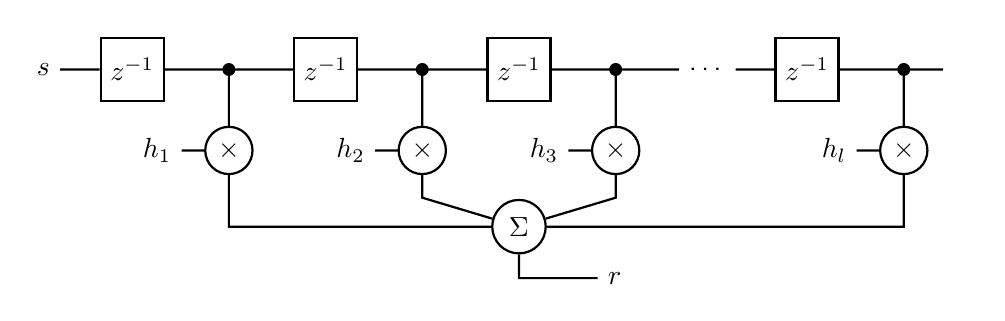
\begin{tikzpicture}[
		dot/.style = {
			circle,
			fill = black, draw = black,
			minimum size = 1.5mm,
			outer sep = 0, inner sep = 0,
		},
		block/.style = {
			rectangle, draw, thick,
			black, fill = white,
			minimum height = 8mm, minimum width = 8mm,
		},
		prod/.style = {
			circle, draw, thick,
			black, fill = white,
			minimum size = 6mm,
			inner sep = 0, outer sep = 0,
		},
		sum/.style = {
			circle, draw, thick,
			black, fill = white,
			minimum size = 4mm,
		},
	]

	\matrix[column sep = 5mm, row sep = 3mm] {
		\node[block] (B0) {\(z^{-1}\)}; & \node[dot] (D0) {}; &
		\node[block] (B1) {\(z^{-1}\)}; & \node[dot] (D1) {}; &
		\node[block] (B2) {\(z^{-1}\)}; & \node[dot] (D2) {}; & \node (dots) {\ldots}; & 
		\node[block] (Bk) {\(z^{-1}\)}; & \node[dot] (Dk) {};
		\\
		& \node[prod] (P0) {\(\times\)}; &
		& \node[prod] (P1) {\(\times\)}; &
		& \node[prod] (P2) {\(\times\)}; & &
		& \node[prod] (Pk) {\(\times\)}; &
		\\
		& & & & \node[sum] (S) {\(\Sigma\)}; \\
	};

	\draw[thick]
		% tapped delayed line
		(B0.west) -- ++(-5mm,0) node[left] {\(s\)}
		(B0.east) -- (D0) -- (B1.west)
		(B1.east) -- (D1) -- (B2.west)
		(B2.east) -- (D2) -- (dots) -- (Bk.west) 
		(Bk.east) -- (Dk) -- ++(5mm,0)
		% taps asd sum
		(D0) -- (P0) |- (S)
		(D1) -- (P1) -- ++(0,-6mm) -- (S)
		(D2) -- (P2) -- ++(0,-6mm) -- (S)
		(Dk) -- (Pk) |- (S)
		% product weights
		(P0.west) -- ++(-3mm,0) node[left] {\(h_1\)}
		(P1.west) -- ++(-3mm,0) node[left] {\(h_2\)}
		(P2.west) -- ++(-3mm,0) node[left] {\(h_3\)}
		(Pk.west) -- ++(-3mm,0) node[left] {\(h_l\)}
		% result
		(S.south) |- ++(1cm,-3mm) node[right] {\(r\)}
	;

\end{tikzpicture}

	\end{figure}
	\begin{equation} 
		h_l(m) = \sum_k c_k(mT) \sinc(l - \tau(mT)/T)
	\end{equation}
\end{frame}


\subsection{Statistical model}

\begin{frame}[fragile]{Statistical model}
  \begin{columns}
    \begin{column}{.5\linewidth}
      \begin{itemize}
        \item Raileigh distribution (NLOS)
        \item Rician distribution (LOS) 
     \end{itemize}
    \end{column}
    \begin{column}{.5\linewidth}
  	  \begin{figure}
  		\centering
  		\resizebox{!}{4cm}{%
  			% vim:set ts=2 sw=2 noet:
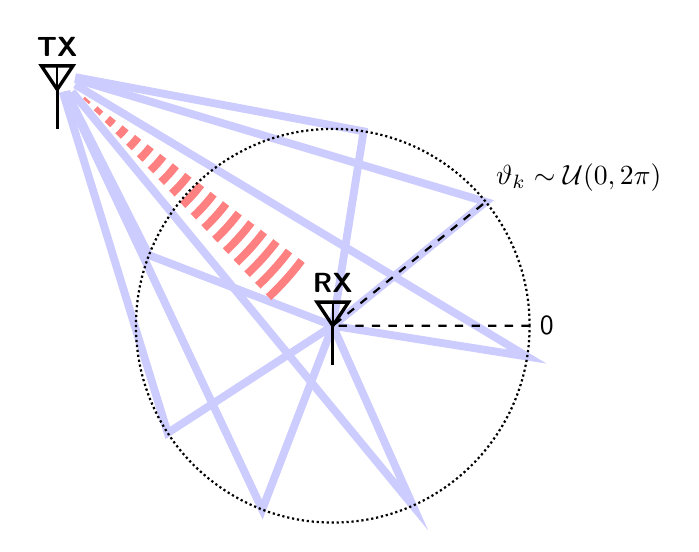
\begin{tikzpicture}[
			antenna/.pic = {
				\draw[very thick] (0,0) -- ++(2mm, 3mm) -- ++(-4mm,0) -- cycle;
				\draw[very thick] (0,0) -- ++(0,-5mm) coordinate (-mast) {};
				\draw[thick] (0,0) -- ++(0,3mm);
				\node[inner sep = 0pt, outer sep = 6pt] (-center) at (0,2mm) {};
			},
	]

	\coordinate (X) at (-3.5,3);

	% antennas
	\draw (X) pic (T) {antenna} node[above = 3mm] {\sffamily\bfseries TX};

	% rays
	\foreach \i [count=\j] in {-2.2,-0.3,1.3,2.7,5.3,7.1,8.3}{
		\draw[blue!20, line width = 1mm]
			(T-center) -- ({30 * \i}:25mm) coordinate (p\j) -- (0,0);
	};

	% angle
	\draw[dashed, thick] (25mm, 0) node[right] {0}
		-- (0,0) -- (p3) node[above right] {\(\vartheta_k \sim \mathcal{U}(0,2\pi)\)};

	% LOS
	\draw[line width = 1mm, red!50,
		decorate, decoration = {
			expanding waves, angle = 5, segment length = 2mm
		}
	] (T-center) -- (-5mm, 5mm);

	% ring und RX antenna
	\draw (0,0) pic (R) {antenna} node[above = 3mm] {\sffamily\bfseries RX};
	\draw[thick, densely dotted] circle (25mm);
	

\end{tikzpicture}

  		}
  	 \end{figure}
    \end{column}
  \end{columns}
\end{frame}





\section{Implementation}

%TODO: Mabe picture Hardware, Bicture GR.

\begin{frame}{Tools}
  \begin{columns}
	\begin{column}{.5\linewidth}
		\begin{itemize}
			\item Software Stack
				\begin{itemize}
					\item GNU Radio
					\item Dear PyGUI
				\end{itemize}
			\item Hardware
			\begin{itemize}
				\item USRP B210
			\end{itemize}
		\end{itemize}
	\end{column}
	\begin{column}{.5\linewidth}
		\begin{figure}
		\centering
		\includegraphics[frame, width = \linewidth]{figures/screenshots/gui_screenshot}
		\end{figure}
	\end{column}
\end{columns}
\end{frame}


\begin{frame}{Blockdiagram}
	\begin{figure}
		\centering
		\resizebox{.9\linewidth}{!}{
			\documentclass[tikz]{standalone}

\usepackage{roboto}
\usepackage{roboto-mono}
\usepackage{tikz}        % Pretty drawings
\usepackage{tikz-3dplot} % More dimensions!
\usetikzlibrary{
	external,
	calc,
	positioning,
	backgrounds,
	decorations.pathreplacing,
	calligraphy,
	decorations.markings,
	matrix,
	arrows,
	patterns,
}
\pgfdeclarelayer{background}
\pgfdeclarelayer{foreground}
\pgfsetlayers{background,main,foreground}

\begin{document}
\documentclass[tikz]{standalone}

\usepackage{roboto}
\usepackage{roboto-mono}
\usepackage{tikz}        % Pretty drawings
\usepackage{tikz-3dplot} % More dimensions!
\usetikzlibrary{
	external,
	calc,
	positioning,
	backgrounds,
	decorations.pathreplacing,
	calligraphy,
	decorations.markings,
	matrix,
	arrows,
	patterns,
}
\pgfdeclarelayer{background}
\pgfdeclarelayer{foreground}
\pgfsetlayers{background,main,foreground}

\begin{document}
\documentclass[tikz]{standalone}

\usepackage{roboto}
\usepackage{roboto-mono}
\usepackage{tikz}        % Pretty drawings
\usepackage{tikz-3dplot} % More dimensions!
\usetikzlibrary{
	external,
	calc,
	positioning,
	backgrounds,
	decorations.pathreplacing,
	calligraphy,
	decorations.markings,
	matrix,
	arrows,
	patterns,
}
\pgfdeclarelayer{background}
\pgfdeclarelayer{foreground}
\pgfsetlayers{background,main,foreground}

\begin{document}
\include{tikz/overview.tex}
\end{document}

\end{document}

\end{document}

		}
		
	\end{figure}
\end{frame}



\subsection{Transmitter and Receiver chain}

\begin{frame}{Transmitter chain}
	
\end{frame}

\begin{frame}{Receiver chain}
	
\end{frame}

\subsection{Channel model}

\begin{frame}{Discrete-time model}
	\begin{figure}
		\centering
		% vim: set ts=2 sw=2 noet:

\newcommand{\makeplot}[6]{%
	\hfill
	\begin{tikzpicture}
		\begin{axis}[
				width  = {\linewidth / 3.5},
				height = {\linewidth / 3.5},
				grid = major,
				xmin = {-#4}, xmax = {#4},
				ymin = {-#4}, ymax = {#4},
				#5
			]

			\addplot[only marks, #6] table[x index = #2, y index = #3] {#1};
		\end{axis}
	\end{tikzpicture}
	\hfill
}

\noindent
\makeplot{figures/data/qpsk_sim_const_static_firblock_nlos_halfsymb.dat}{0}{1}{4}{
	ylabel = {Channel with ISI},
	yticklabel style = {
		text width = 2.25em,
		align = right,
	},
	title = {},
}{magenta}
\makeplot{figures/data/qpsk_sim_const_static_firblock_los_halfsymb.dat}{0}{1}{4}{title = {},}{magenta}
\makeplot{figures/data/qpsk_sim_const_static_firblock_los_vec.dat}{0}{1}{4}{title = {},}{magenta}
\newline

\noindent
\makeplot{figures/data/qpsk_sim_const_static_firblock_nlos_halfsymb.dat}{2}{3}{4}{%
	ylabel = {Synchronized},
	yticklabel style = {
		text width = 2.25em,
		align = right,
	},
}{magenta!80!blue}
\makeplot{figures/data/qpsk_sim_const_static_firblock_los_halfsymb.dat}{2}{3}{4}{}{magenta!80!blue}
\makeplot{figures/data/qpsk_sim_const_static_firblock_los_vec.dat}{2}{3}{4}{}{magenta!80!blue}
\newline

\noindent
\makeplot{figures/data/qpsk_sim_const_static_firblock_nlos_halfsymb.dat}{4}{5}{1}{%
	ylabel = {Equalized},
	yticklabel style = {
		text width = 2.25em,
		align = right,
	},
}{magenta!60!blue}
\makeplot{figures/data/qpsk_sim_const_static_firblock_los_halfsymb.dat}{4}{5}{1}{}{magenta!60!blue}
\makeplot{figures/data/qpsk_sim_const_static_firblock_los_vec.dat}{4}{5}{1}{}{magenta!60!blue}
\newline

\noindent
\makeplot{figures/data/qpsk_sim_const_static_firblock_nlos_halfsymb.dat}{6}{7}{1}{%
	ylabel = {Locked},
	yticklabel style = {
		text width = 2.25em,
		align = right,
	},
}{magenta!40!blue}
\makeplot{figures/data/qpsk_sim_const_static_firblock_los_halfsymb.dat}{6}{7}{1}{}{magenta!40!blue}
\makeplot{figures/data/qpsk_sim_const_static_firblock_los_vec.dat}{6}{7}{1}{}{magenta!40!blue}
\newline


	\end{figure}
	the 1 tap model the fading tap was \(0.2\delta(n - 0.25)\), and for the 4 tap model uses \(0.2 \delta(n - 0.25) + 0.08 \delta(n - 3.25) + 0.5 \delta(n - 4) + 0.4 \delta(n - 6.3)\). In both cases the delays are given in samples.
\end{frame}

\begin{frame}{Statistical model}
	
\end{frame}

\section{Conclusion}

\begin{frame}{Further steps}
	
\end{frame}

\section{Measurement/Demonstration}

%%Tools


\end{document}

% vim:et:ts=2:sw=2:wrap:nolinebreak:
